\DiaryEntry{Pentagonal Numbers}{2018-02-08}{Maths}

We have pentagrams as in the Figure below with different size $n$. 

\begin{figure}[H]
	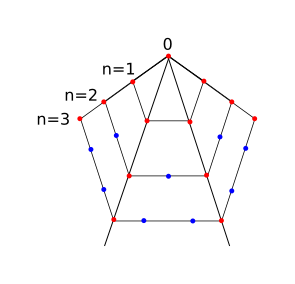
\includegraphics[scale=1.3]{images/pentagon_numbers.png}
\end{figure}

The task is to count all points $p(n)$ which are contained in the pentagrams of size up to (and including $n$). According to the Figure, $p(1) = 5, p(2) = 12, p(3) = 22...$. Note that the definition of $n$ is slightly different than the Wikipedia one.

\subsection{Solution via Counting}

In order to solve this, we first count the red dots $p_1(n)$ in the Figure as $p_1(n) = 1 + 4n$.

The number $p_2(n)$ of the blue dots is a bit more tricky; we have

\bee
p_2(n) = 3 \sum_{k=1}^{n-1} k = 3 \frac{n(n-1)}{2}
\eee

and in total, we obtain

\be
\label{eq:2018-02-08-1}
p(n) = 1 + 4n + 3 \frac{n(n-1)}{2} = \cdots = \frac{3n^2 + 5n+2}{2}
\ee

The Wikipedia solution starts at $n=1$; i.e. we have $n \rightarrow n-1$. Applying this substitution, we obtain

\bee
\tilde{p}(n) = \frac{3(n-1)^2 + 5(n-1) + 2}{2} = \cdots = \frac{3n^2-n}{2}
\eee


\subsection{Solution via Sequence Values}

Another - probably more brute-force - option is to "guess" that $p(n)$ scales with $n^2$. Then we can make the following ansatz

\bee
p(n) = An^2 + Bn + C
\eee

and with $p(1) = 5, p(2) = 12, p(3) = 22$, we obtain a linear system of equations for $A,B,C$. We can solve this and arrive at the expression \eqref{eq:2018-02-08-1}.


Use Maxima to solve the equation system:


\begin{verbatim}
(%i1)	linsolve([a+b+c=5, 4*a+2*b+c=12, 9*a+3*b+c=22], [a,b,c]);
(%o1)	[a=3/2,b=5/2,c=1]
\end{verbatim}


